% Copyright 2003 by Till Tantau <tantau@cs.tu-berlin.de>.
%
% This program can be redistributed and/or modified under the terms
% of the LaTeX Project Public License Distributed from CTAN
% archives in directory macros/latex/base/lppl.txt.


\section{Constructing Paths}

\subsection{Overview}

The ``basic entity of drawing'' in \pgfname\ is the \emph{path}. A
path consists of several parts, each of which is either a closed or
open curve. An open curve has a starting point and an end point and,
in between, consists of several \emph{segments}, each of which is
either a straight line or a B�zier curve. Here is an example of a
path (in red) consisting of two parts, one open, one closed:

\begin{codeexample}[]
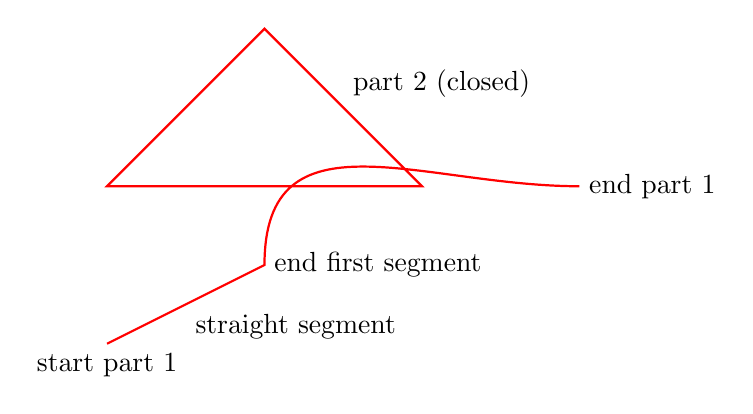
\begin{tikzpicture}[scale=2]
  \draw[thick,red]
       (0,0) coordinate (a)
    -- coordinate (ab) (1,.5) coordinate (b)
    .. coordinate (bc) controls +(up:1cm) and +(left:1cm) .. (3,1)  coordinate (c)
       (0,1) -- (2,1) -- coordinate (x) (1,2) -- cycle;

  \draw (a)  node[below] {start part 1}
        (ab) node[below right] {straight segment}
        (b)  node[right] {end first segment}
        (c)  node[right] {end part 1}
        (x)  node[above right]  {part 2 (closed)};        
\end{tikzpicture}
\end{codeexample}

A path, by itself, has no ``effect,'' that is, it does not leave any
marks on the page. It is just a set of points on the plane. However,
you can \emph{use} a path in different ways. The most natural actions
are \emph{stroking} (also known as \emph{drawing}) and
\emph{filling}. Stroking can be imagined as picking up a pen of a
certain diameter and ``moving it along the path.'' Filling means that
everything ``inside'' the path is filled with a uniform
color. Naturally, the open parts of a path must first be closed before
a path can be filled.

In \pgfname, there are numerous commands for constructing paths, all
of which start with |\pgfpath|. There are also commands for
\emph{using} paths, though most operations can be performed by calling
|\pgfusepath| with an appropriate parameter.

As a side-effect, the path construction commands keep track of two
bounding boxes. One is the bounding box for the current path, the
other is a bounding box for all paths in the current picture. See
Section~\ref{section-bb} for more details.

Each path construction command extends the current path in some
way. The ``current path'' is a global entity that persists across
\TeX\ groups. Thus, between calls to the path construction commands
you can perform arbitrary computations and even open and closed \TeX\
groups. The current path only gets ``flushed'' when the |\pgfusepath|
command is called (or when the soft-path subsystem is used directly,
see Section~\ref{section-soft-paths}).

\subsection{The Move-To Path Operation}

The most basic operation is the move-to operation. It must be given at
the beginning of paths, though some path construction command (like
|\pgfpathrectangle|) generate move-tos implicitly. A move-to operation
can also be used to start a new part of a path. 

\begin{command}{\pgfpathmoveto\marg{coordinate}}
  This command expects a \pgfname-coordinate like |\pgfpointorigin| as
  its parameter. When the current path is empty, this operation will
  start the path at the given \meta{coordinate}. If a path has already
  been partly constructed, this command will end the current part of
  the path and start a new one.
\begin{codeexample}[]
\begin{pgfpicture}
  \pgfpathmoveto{\pgfpointorigin}
  \pgfpathlineto{\pgfpoint{1cm}{1cm}}
  \pgfpathlineto{\pgfpoint{2cm}{1cm}}
  \pgfpathlineto{\pgfpoint{3cm}{0.5cm}}
  \pgfpathlineto{\pgfpoint{3cm}{0cm}}
  \pgfsetfillcolor{examplefill}
  \pgfusepath{fill,stroke}
\end{pgfpicture}
\end{codeexample}
\begin{codeexample}[]
\begin{pgfpicture}
  \pgfpathmoveto{\pgfpointorigin}
  \pgfpathlineto{\pgfpoint{1cm}{1cm}}
  \pgfpathlineto{\pgfpoint{2cm}{1cm}}
  \pgfpathmoveto{\pgfpoint{2cm}{1cm}} % New part
  \pgfpathlineto{\pgfpoint{3cm}{0.5cm}}
  \pgfpathlineto{\pgfpoint{3cm}{0cm}}
  \pgfsetfillcolor{examplefill}
  \pgfusepath{fill,stroke}
\end{pgfpicture}
\end{codeexample}
  The command will apply the current coordinate transformation matrix
  to \meta{coordinate} before using it.

  The command will update the bounding box of the current path and
  picture, if necessary. 
\end{command}


\subsection{The Line-To Path Operation}

\begin{command}{\pgfpathlineto\marg{coordinate}}
  This command extends the current path in a straight line to the
  given \meta{coordinate}. If this command is given at the beginning
  of path without any other path construction command given before (in
  particular without a move-to operation), the \TeX\ file may compile
  without an error message, but a viewer application may display an
  error message when trying to render the picture. 
\begin{codeexample}[]
\begin{pgfpicture}
  \pgfpathmoveto{\pgfpointorigin}
  \pgfpathlineto{\pgfpoint{1cm}{1cm}}
  \pgfpathlineto{\pgfpoint{2cm}{1cm}}
  \pgfsetfillcolor{examplefill}
  \pgfusepath{fill,stroke}
\end{pgfpicture}
\end{codeexample}
  The command will apply the current coordinate transformation matrix
  to \meta{coordinate} before using it.

  The command will update the bounding box of the current path and
  picture, if necessary. 
\end{command}


\subsection{The Curve-To Path Operation}

\begin{command}{\pgfpathcurveto\marg{support 1}\marg{support 2}\marg{coordinate}}
  This command extends the current path with a B�zier curve from the
  last point of the path to  \meta{coordinate}. The \meta{support 1}
  and \meta{support 2} are the first and second support point of the
  B�zier curve. For more information on B�zier curve, please consult a
  standard textbook on computer graphics.

  Like the line-to command, this command may not be the first path
  construction command in a path.
\begin{codeexample}[]
\begin{pgfpicture}
  \pgfpathmoveto{\pgfpointorigin}
  \pgfpathcurveto
    {\pgfpoint{1cm}{1cm}}{\pgfpoint{2cm}{1cm}}{\pgfpoint{3cm}{0cm}}
  \pgfsetfillcolor{examplefill}
  \pgfusepath{fill,stroke}
\end{pgfpicture}
\end{codeexample}
  The command will apply the current coordinate transformation matrix
  to \meta{coordinate} before using it.

  The command will update the bounding box of the current path and
  picture, if necessary. However, the bounding box is simply made
  large enough such that it encompasses all of the support points and
  the \meta{coordinate}. This will guarantee that the curve is
  completely inside the bounding box, but the bounding box will
  typically be quite a bit too large. It is not clear (to me) how this 
  can be avoided without resorting to ``some serious math'' in order
  to calculate a precise bounding box. 
\end{command}


\subsection{The Close Path Operation}

\begin{command}{\pgfpathclose}
  This command closes the current part of the path by appending a
  straight line to the start point of the current part. Note that there
  \emph{is} a difference between closing a path and using the line-to
  operation to add a straight line to the start of the current
  path. The difference is demonstrated by the upper corners of the triangles
  in the following example: 
\begin{codeexample}[]
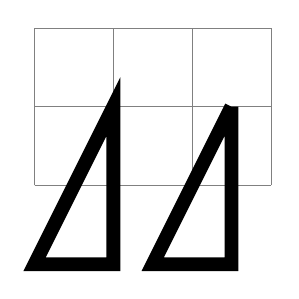
\begin{tikzpicture}
  \draw[help lines] (0,0) grid (3,2);
  \pgfsetlinewidth{5pt}
  \pgfpathmoveto{\pgfpoint{1cm}{1cm}}
  \pgfpathlineto{\pgfpoint{0cm}{-1cm}}
  \pgfpathlineto{\pgfpoint{1cm}{-1cm}}
  \pgfpathclose
  \pgfpathmoveto{\pgfpoint{2.5cm}{1cm}}
  \pgfpathlineto{\pgfpoint{1.5cm}{-1cm}}
  \pgfpathlineto{\pgfpoint{2.5cm}{-1cm}}
  \pgfpathlineto{\pgfpoint{2.5cm}{1cm}}
  \pgfusepath{stroke}
\end{tikzpicture}
\end{codeexample}
\end{command}


\subsection{Arc, Ellipse and Circle Path Operations}

The path construction commands that we have discussed up to now are
sufficient to create all paths that can be created ``at all.''
However, it is useful to have special commands to create certain
shapes, like circles, that arise often in practice.

In the following, the commands for adding (parts of) (transformed)
circles to a path are described.

\begin{command}{\pgfpatharc\marg{start angle}\marg{end
      angle}\marg{radius}}
  This command appends a part of a circle (or an ellipse) to the current
  path. Imaging the curve between \meta{start angle} and \meta{end
    angle} on a circle of radius \meta{radius} (if $\meta{start angle}
  < \meta{end angle}$, the curve goes around the circle
  counterclockwise, otherwise clockwise). This curve is now moved such
  that the point where the curve starts is the previous last point of the
  path. Note that this command will \emph{not} start a new part of the
  path, which is important for example for filling purposes. 

\begin{codeexample}[]
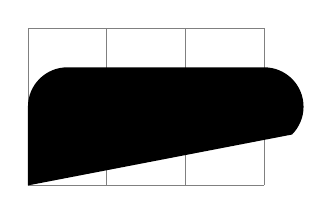
\begin{tikzpicture}
  \draw[help lines] (0,0) grid (3,2);
  \pgfpathmoveto{\pgfpointorigin}
  \pgfpathlineto{\pgfpoint{0cm}{1cm}}
  \pgfpatharc{180}{90}{.5cm}
  \pgfpathlineto{\pgfpoint{3cm}{1.5cm}}
  \pgfpatharc{90}{-45}{.5cm}
  \pgfusepath{fill}
\end{tikzpicture}
\end{codeexample}

  Saying |\pgfpatharc{0}{360}{1cm}| ``nearly'' gives you a full
  circle. The ``nearly'' refers to the fact that the circle will not
  be closed. You can close it using |\pgfpathclose|.

  The \meta{radius} need not always be a single \TeX\
  dimension. Instead, it can also contain a slash, in which case it
  must consist of two dimensions separated by this slash. In this
  case the first dimension is the $x$-radius and the second the
  $y$-radius of the ellipse from which the curve is taken:  

\begin{codeexample}[]
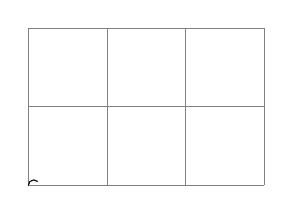
\begin{tikzpicture}
  \draw[help lines] (0,0) grid (3,2);
  \pgfpathmoveto{\pgfpointorigin}
  \pgfpatharc{180}{45}{2cm/1cm}
  \pgfusepath{draw}
\end{tikzpicture}
\end{codeexample}

  The axes of the circle or ellipse from which the arc is ``taken''
  always point up and right. However, the current coordinate
  transformation matrix will have an effect on the arc. This can be
  used to, say, rotate an arc:

\begin{codeexample}[]
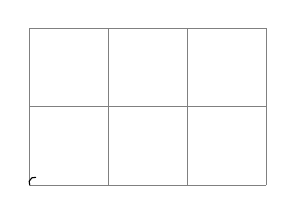
\begin{tikzpicture}
  \draw[help lines] (0,0) grid (3,2);
  \pgftransformrotate{30}
  \pgfpathmoveto{\pgfpointorigin}
  \pgfpatharc{180}{45}{2cm/1cm}
  \pgfusepath{draw}
\end{tikzpicture}
\end{codeexample}

  The command will update the bounding box of the current path and
  picture, if necessary. Unless rotation or shearing transformations
  are applied, the bounding box will be tight.
\end{command}

\begin{command}{\pgfpathellipse\marg{center}\marg{first
      axis}\marg{second axis}}
  The effect of this command is to append an ellipse to the current
  path (if the path is not empty, a new part is started). The
  ellipse's center will be \meta{center} and \meta{first axis} and
  \meta{second axis} are the axis \emph{vectors}. The same effect as
  this command can also be achieved using an appropriate sequence of
  move-to, arc, and close operations, but this command is easier and
  faster. 

\begin{codeexample}[]
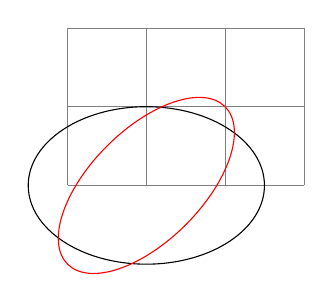
\begin{tikzpicture}
  \draw[help lines] (0,0) grid (3,2);
  \pgfpathellipse{\pgfpoint{1cm}{0cm}}
                 {\pgfpoint{1.5cm}{0cm}}
                 {\pgfpoint{0cm}{1cm}}
  \pgfusepath{draw}
  \color{red}               
  \pgfpathellipse{\pgfpoint{1cm}{0cm}}
                 {\pgfpoint{1cm}{1cm}}
                 {\pgfpoint{-0.5cm}{0.5cm}}
  \pgfusepath{draw}
\end{tikzpicture}
\end{codeexample}

  The command will apply coordinate transformations to all coordinates
  of the ellipse. However, the coordinate transformations are applied
  only after the ellipse is ``finished conceptually.'' Thus, a
  transformation of 1cm to the right will simply shift the ellipse one
  centimeter to the right; it will not add 1cm to the $x$-coordinates
  of the two axis vectors.

  The command will update the bounding box of the current path and
  picture, if necessary. 
\end{command}

\begin{command}{\pgfpathcirlce\marg{center}\marg{radius}}
  A shorthand for |\pgfpathellipse| applied to \meta{center} and the
  two axis vectors $(\meta{radius},0)$ and $(0,\meta{radius})$. 
\end{command}


\subsection{Rectangle Path Operations}

Another shape that arises frequently is the rectangle. Two commands
can be used to add a rectangle to the current path. Both commands will
start a new part of the path.


\begin{command}{\pgfpathrectangle\marg{corner}\marg{diagonal vector}}
  Adds a rectangle to the path whose one corner is \meta{corner} and
  whose opposite corner is given by $\meta{corner} + \meta{diagonal
    vector}$.

\begin{codeexample}[]
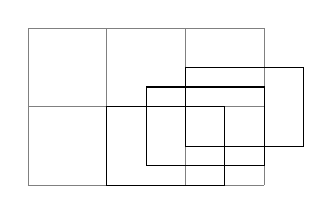
\begin{tikzpicture}
  \draw[help lines] (0,0) grid (3,2);
  \pgfpathrectangle{\pgfpoint{1cm}{0cm}}{\pgfpoint{1.5cm}{1cm}}
  \pgfpathrectangle{\pgfpoint{1.5cm}{0.25cm}}{\pgfpoint{1.5cm}{1cm}}
  \pgfpathrectangle{\pgfpoint{2cm}{0.5cm}}{\pgfpoint{1.5cm}{1cm}}
  \pgfusepath{draw}
\end{tikzpicture}
\end{codeexample}
  The command will apply coordinate transformations and update the
  bounding boxes tightly.
\end{command}


\begin{command}{\pgfpathrectanglecorners\marg{corner}\marg{opposite corner}}
  Adds a rectangle to the path whose two opposing corners are
  \meta{corner} and \meta{opposite corner}.
\begin{codeexample}[]
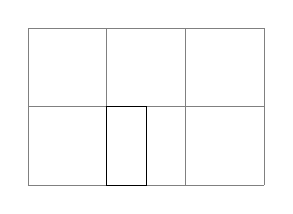
\begin{tikzpicture}
  \draw[help lines] (0,0) grid (3,2);
  \pgfpathrectanglecorners{\pgfpoint{1cm}{0cm}}{\pgfpoint{1.5cm}{1cm}}
  \pgfusepath{draw}
\end{tikzpicture}
\end{codeexample}
  The command will apply coordinate transformations and update the
  bounding boxes tightly.
\end{command}



\subsection{The Grid Path Operation}

\begin{command}{\pgfpathgrid\oarg{options}\marg{lower left}\marg{upper right}}
  Appends a grid to the current path. That is, a (possibly large)
  number of parts are added to the path, each part consisting of a
  single horizontal or vertical straight line segment.

  Conceptually, the origin is part of the grid and the grid is clipped 
  to the rectangle specified by the \meta{lower left} and
  the \meta{upper right} corner. However, no clipping occurs (this
  command just adds parts to the current path). Rather, the points
  where the lines enter and leave the ``clipping area'' are computed
  and used to add simple lines to the current path.

  Allowed \meta{options} are:
  \begin{itemize}
    \itemoption{stepx}|=|\meta{dimension}
    Sets the horizontal stepping to \meta{dimension}. Default is 1cm.
    \itemoption{stepy}|=|\meta{dimension}
    Sets the vertical stepping to \meta{dimension}. Default is 1cm.
    \itemoption{step}|=|\meta{vector}
    Sets the horizontal stepping to the $x$-coordinate of
    \meta{vector} and the vertical stepping to its $y$-coordinate.
  \end{itemize}
\begin{codeexample}[]
\begin{pgfpicture}
  \pgfsetlinewidth{0.8pt}
  \pgfpathgrid[step={\pgfpoint{1cm}{1cm}}]
    {\pgfpoint{-3mm}{-3mm}}{\pgfpoint{33mm}{23mm}}
  \pgfusepath{stroke}
  \pgfsetlinewidth{0.4pt}
  \pgfpathgrid[stepx=1mm,stepy=1mm]
    {\pgfpoint{-1.5mm}{-1.5mm}}{\pgfpoint{31.5mm}{21.5mm}}
  \pgfusepath{stroke}
\end{pgfpicture}
\end{codeexample}
  The command will apply coordinate transformations and update the
  bounding boxes tightly. As for ellipses, the transformations are
  applied to the ``conceptually finished'' grid. 
\begin{codeexample}[]
\begin{pgfpicture}
  \pgftransformrotate{10}
  \pgfpathgrid[stepx=1mm,stepy=2mm]{\pgfpoint{0mm}{0mm}}{\pgfpoint{30mm}{30mm}}
  \pgfusepath{stroke}
\end{pgfpicture}
\end{codeexample}
\end{command}


\subsection{The Parabola Path Operation}

\begin{command}{\pgfpathparabola\marg{bend vector}\marg{end vector}}
  This command appends two half-parabolas to the  current path. The
  first starts at the current point and ends at the current point plus
  \meta{bend vector}. At his point, it has its bend. The second half
  parabola starts at that bend point and end at point that is given by
  the bend plus \meta{end vector}.

  If you set \meta{end vector} to the null vector, you append only a
  half parabola that goes from the current point to the bend; by
  setting \meta{bend vector} to the null vector, you append only a
  half parabola that goes to current point plus \meta{end vector} and
  has its bend at the current point.

  It is not possible to use this command to draw a part of a parabola
  that does not contain the bend.

\begin{codeexample}[]
\begin{pgfpicture}
  % Half-parabola going ``up and right''
  \pgfpathmoveto{\pgfpointorigin}
  \pgfpathparabola{\pgfpointorigin}{\pgfpoint{2cm}{4cm}}
  \color{red}
  \pgfusepath{stroke}

  % Half-parabola going ``down and right''
  \pgfpathmoveto{\pgfpointorigin}
  \pgfpathparabola{\pgfpoint{-2cm}{4cm}}{\pgfpointorigin}
  \color{blue}
  \pgfusepath{stroke}

  % Full parabola
  \pgfpathmoveto{\pgfpoint{-2cm}{2cm}}
  \pgfpathparabola{\pgfpoint{1cm}{-1cm}}{\pgfpoint{2cm}{4cm}}
  \color{orange}
  \pgfusepath{stroke}
\end{pgfpicture}
\end{codeexample}
  The command will apply coordinate transformations and update the
  bounding boxes.
\end{command}


\subsection{Sine and Cosine Path Operations}

Sine and cosine curves often need to be drawn and the following commands
may help with this. However, they only allow you to append sine and
cosine curves in intervals that are multiples of $\pi/2$.

\begin{command}{\pgfpathsine\marg{vector}}
  This command appends a sine curve in the interval $[0,\pi/2]$ to the
  current path. The sine curve is squeezed or stretched such that the
  curve starts at the current point and ends at the current point plus
  \meta{vector}.
\begin{codeexample}[]
\begin{tikzpicture}
  \draw[help lines] (0,0) grid (3,1);
  \pgfpathmoveto{\pgfpoint{1cm}{0cm}}
  \pgfpathsine{\pgfpoint{1cm}{1cm}}
  \pgfusepath{stroke}

  \color{red}
  \pgfpathmoveto{\pgfpoint{1cm}{0cm}}
  \pgfpathsine{\pgfpoint{-2cm}{-2cm}}
  \pgfusepath{stroke}
\end{tikzpicture}
\end{codeexample}
  The command will apply coordinate transformations and update the
  bounding boxes.  
\end{command}

\begin{command}{\pgfpathcosine\marg{vector}}
  This command appends a cosine curve in the interval $[0,\pi/2]$ to the
  current path. The curve is squeezed or stretched such that the
  curve starts at the current point and ends at the current point plus
  \meta{vector}. Using several sine and cosine operations in sequence
  allows you to produce a complete sine or cosine curve
\begin{codeexample}[]
\begin{pgfpicture}
  \pgfpathmoveto{\pgfpoint{0cm}{0cm}}
  \pgfpathsine{\pgfpoint{1cm}{1cm}}
  \pgfpathcosine{\pgfpoint{1cm}{-1cm}}
  \pgfpathsine{\pgfpoint{1cm}{-1cm}}
  \pgfpathcosine{\pgfpoint{1cm}{1cm}}
  \pgfsetfillcolor{examplefill}
  \pgfusepath{fill,stroke}
\end{pgfpicture}
\end{codeexample}
  The command will apply coordinate transformations and update the
  bounding boxes.  
\end{command}


\subsection{Plot Path Operations}

There exist several commands for appending
plots to a path. These
commands are available through the package |pgfbaseplot|. They are
documented in Section~\ref{section-plots}.


\subsection{Rounded Corners}

Normally, when you connect two straight line segments or when you
connect two curves that end and start ``at different angles'' you get
``sharp corners'' between the lines or curves. In some cases it is
desirable to produce ``rounded corners'' instead. Thus, the lines
or curves should be shortened a bit and then connected by arcs.

\pgfname\ offers an easy way to achieve this effect, by calling the
following two commands.

\begin{command}{\pgfsetcornersarced\marg{point}}
  This command causes all subsequent corners to be replaced by little
  arcs. The effect of this command lasts till the end of the current
  \TeX\ scope.

  The \meta{point} dictates how large the corner arc will be. Consider
  a corner made by two lines $l$ and~$r$ and assume that the line $l$
  comes first on the path. The $x$-dimension of the \meta{point}
  decides by how much the line~$l$ will be shortened, the
  $y$-dimension of \meta{point} decides by how much the line $r$ will
  be shortened. Then, the shortened lines are connected by an arc.

\begin{codeexample}[]
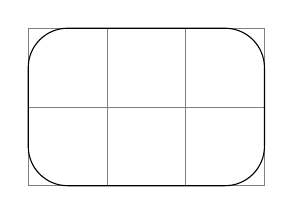
\begin{tikzpicture}
  \draw[help lines] (0,0) grid (3,2);

  \pgfsetcornersarced{\pgfpoint{5mm}{5mm}}
  \pgfpathrectanglecorners{\pgfpointorigin}{\pgfpoint{3cm}{2cm}}
  \pgfusepath{stroke}
\end{tikzpicture}
\end{codeexample}

\begin{codeexample}[]
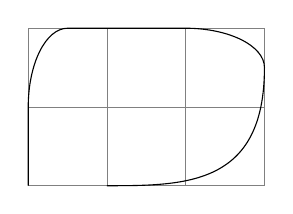
\begin{tikzpicture}
  \draw[help lines] (0,0) grid (3,2);

  \pgfsetcornersarced{\pgfpoint{10mm}{5mm}}
  % 10mm entering,
  % 5mm leaving.
  \pgfpathmoveto{\pgfpointorigin}
  \pgfpathlineto{\pgfpoint{0cm}{2cm}}
  \pgfpathlineto{\pgfpoint{3cm}{2cm}}
  \pgfpathcurveto
    {\pgfpoint{3cm}{0cm}}
    {\pgfpoint{2cm}{0cm}}
    {\pgfpoint{1cm}{0cm}}
  \pgfusepath{stroke}
\end{tikzpicture}
\end{codeexample}

  If the $x$- and $y$-coordinates of \meta{point} are the same and the
  corner is a right angle, you will get a perfect quarter circle
  (well, not quite perfect, but perfect up to six decimals). When the
  angle is not $90^\circ$, you only get a fair approximation.

  More or less ``all'' corners will be rounded, even the corner
  generated by a |\pgfpathclose| command. (The author is a bit proud
  of this feature.)
  
\begin{codeexample}[]
\begin{pgfpicture}
  \pgfsetcornersarced{\pgfpoint{4pt}{4pt}}
  \pgfpathmoveto{\pgfpointpolar{0}{1cm}}
  \pgfpathlineto{\pgfpointpolar{72}{1cm}}
  \pgfpathlineto{\pgfpointpolar{144}{1cm}}
  \pgfpathlineto{\pgfpointpolar{216}{1cm}}
  \pgfpathlineto{\pgfpointpolar{288}{1cm}}
  \pgfpathclose
  \pgfusepath{stroke}
\end{pgfpicture}
\end{codeexample}

  To return to normal (unrounded) corners, use
  |\pgfsetcornersarced{\pgfpointorigin}|.

  Note that the rounding will produce strange and undesirable effects
  if the lines at the corners are too short. In this case the
  shortening may cause the lines to ``suddenly extend over the other
  end'' which is rarely desirable. 
\end{command}




\subsection{Internal Tracking of Bounding Boxes for Paths and Pictures}

\label{section-bb}

\makeatletter

The path construction commands keep track of two bounding boxes: One
for the current path, which is reset whenever the path is used and
thereby flushed, and a bounding box for the current |{pgfpicture}|. 

The bounding boxes are not accessible by ``normal'' macros. Rather,
two sets of four dimension variables are used for this, all of which
contain the letter~|@|.

\begin{textoken}{\pgf@pathminx}
  The minimum $x$-coordinate ``mentioned'' in the current
  path. Initially, this is set to $16000$pt.
\end{textoken}

\begin{textoken}{\pgf@pathmaxx}
  The maximum $x$-coordinate ``mentioned'' in the current
  path. Initially, this is set to $-16000$pt.
\end{textoken}

\begin{textoken}{\pgf@pathminy}
  The minimum $y$-coordinate ``mentioned'' in the current
  path. Initially, this is set to $16000$pt.
\end{textoken}

\begin{textoken}{\pgf@pathmaxy}
  The maximum $y$-coordinate ``mentioned'' in the current
  path. Initially, this is set to $-16000$pt.
\end{textoken}

\begin{textoken}{\pgf@picminx}
  The minimum $x$-coordinate ``mentioned'' in the current
  picture. Initially, this is set to $16000$pt.
\end{textoken}

\begin{textoken}{\pgf@picmaxx}
  The maximum $x$-coordinate ``mentioned'' in the current
  picture. Initially, this is set to $-16000$pt.
\end{textoken}

\begin{textoken}{\pgf@picminy}
  The minimum $y$-coordinate ``mentioned'' in the current
  picture. Initially, this is set to $16000$pt.
\end{textoken}

\begin{textoken}{\pgf@picmaxy}
  The maximum $y$-coordinate ``mentioned'' in the current
  picture. Initially, this is set to $-16000$pt.
\end{textoken}


Each time a path construction command is called, the above variables
are (globally) updated. To facilitate this, you can use the following
command:

\begin{command}{\pgf@protocolsizes\marg{x-dimension}\marg{y-dimension}}
  Updates all of the above dimension in such a way that the point
  specified by the two arguments is inside both bounding boxes. For
  the picture's bounding box this updating occurs only if
  |\ifpgf@relevantforpicturesize| is true, see below.
\end{command}

For the bounding box of the picture it is not always desirable that
every path construction command affects this bounding box. For
example, if you have just used a clip command, you do not want anything
outside the clipping area to affect the bounding box. For this reason,
there exists a special ``\TeX\ if'' that (locally) decides whether
updating should be applied to the picture's bounding box. Clipping
will set this if to false, as will certain other commands.

\begin{command}{\pgf@relevantforpicturesizefalse}
  Suppresses updating of the picture's bounding box.
\end{command}

\begin{command}{\pgf@relevantforpicturesizetrue}
  Causes updating of the picture's bounding box.
\end{command}

